%%%%%%%%%%%%%%%%%%%%%%%%%%%%%%%%%%%%%%%%%%%%%%%%%%%%%%%%%%%%%%%%%%%%%%%%%%%%%%%%
% DAXFS: A Lock-Free Shared Filesystem for CXL Disaggregated Memory
% USENIX FAST
%%%%%%%%%%%%%%%%%%%%%%%%%%%%%%%%%%%%%%%%%%%%%%%%%%%%%%%%%%%%%%%%%%%%%%%%%%%%%%%%

\documentclass[letterpaper,twocolumn,10pt]{article}
\usepackage{usenix-2020-09}

\usepackage{tikz}
\usetikzlibrary{arrows.meta,positioning,fit,calc,patterns,decorations.pathreplacing}
\usepackage{amsmath}
\usepackage{booktabs}
\usepackage{listings}
\usepackage{xspace}
\usepackage{multirow}
\usepackage{graphicx}

\lstset{
  basicstyle=\ttfamily\small,
  breaklines=true,
  columns=flexible,
  language=C,
  morekeywords={__le32,__le64,u8,u16,u32,u64,cmpxchg,uint64_t,uint32_t},
}

\newcommand{\daxfs}{\textsc{DaxFS}\xspace}
\newcommand{\ie}{\textit{i.e.}\xspace}
\newcommand{\eg}{\textit{e.g.}\xspace}
% Symbols drawn via TikZ to avoid loading cmsy10.pfb (corrupted in some environments)
\newcommand{\cmark}{\tikz[baseline=-0.5ex,scale=0.7]\draw[thick,green!60!black](0,0.1)--(0.1,0)--(0.3,0.25);}
\newcommand{\xmark}{\tikz[baseline=-0.4ex,scale=0.7]{\draw[thick,red!70!black](0,0)--(0.22,0.22);\draw[thick,red!70!black](0,0.22)--(0.22,0);}}
\newcommand{\todo}[1]{[TODO: #1]}

%-------------------------------------------------------------------------------
\begin{document}
%-------------------------------------------------------------------------------

\date{}

\title{\Large \bf DAXFS: A Lock-Free Shared Filesystem\\
  for Multikernel and CXL Shared Memory}

\author{
{\rm Cong Wang}\\
Multikernel Technologies, Inc.\\
cwang@multikernel.io
\and
{\rm Yiwei Yang}\\
UC Santa Cruz\\
yyang363@ucsc.edu
\and
{\rm Yusheng Zheng}\\
UC Santa Cruz\\
yzhen165@ucsc.edu
} % end author

\maketitle

%-------------------------------------------------------------------------------
\begin{abstract}
%-------------------------------------------------------------------------------
Multi-tenant hosts increasingly run as multiple independent operating
system instances over shared physical memory: multikernels today, and
CXL~3.0 multi-host configurations as the hardware matures.  Such
instances commonly launch containers from a common base image, yet no
existing filesystem lets them share one writable copy.  Per-instance
filesystems duplicate the image and its cache $N$ times, and the one
system that targets shared memory, FamFS, restricts clients to a
read-only, single-master model.
We present \daxfs, a Linux filesystem for shared memory that uses the
hardware-coherent \texttt{cmpxchg} as its sole coordination primitive,
with no locks, logs, journals, or central coordinator.  A CAS-based
hash overlay provides lock-free concurrent writes; a base-plus-overlay
layout shares one read-only image with per-instance copy-on-write; and
for datasets larger than the shared region, a cooperative shared cache
with a decentralized clock eviction algorithm (MH-clock) demand-pages
data into shared memory once for all instances.  \daxfs requires
hardware-coherent atomics only on a small, few-megabyte coordination
region, which fits within CXL's bounded coherent region.
We evaluate \daxfs on real multikernel hardware, where multiple Linux
kernels share one physical memory region with genuine hardware atomics,
and characterize the CXL generalization by emulation.  \daxfs reduces
the memory cost of running $N$ instances of a shared base image from
$N$ copies to one (\todo{E1 numbers}), sustains correct lock-free
cross-kernel coordination under contention (\todo{E2 CAS accuracy}),
and adds negligible single-instance overhead over tmpfs
(\todo{E5 numbers}).

\end{abstract}

%-------------------------------------------------------------------------------
\section{Introduction}
\label{sec:intro}
%-------------------------------------------------------------------------------

Modern multi-tenant hosts increasingly run not as a single operating
system but as several independent OS instances over the same physical
memory.  Multikernel systems partition one machine into multiple Linux
kernels on disjoint cores~\cite{baumann09:multikernel,barbalace15:popcorn},
and CXL~3.0~\cite{cxl22:spec} extends the same shared-memory model
across machines.  In both, a recurring workload is identical: each
instance launches containers, and those containers are built from
common base images.

A container image is a filesystem, not a byte array.  A container
runtime mounts a root filesystem and performs path lookups, opens,
reads, and permission checks; it cannot consume raw shared memory
directly.  So when $N$ instances run containers from the same base
image, each instance instantiates its own filesystem over that image,
and the result is $N$ redundant copies of identical data in memory,
plus $N$ independent caches of it.  This duplication wastes the very
capacity that shared memory is meant to pool, and it grows linearly
with the number of instances.

No existing filesystem removes this duplication while remaining
writable (Table~\ref{tab:feature-matrix}).  Per-instance DAX
filesystems~\cite{xu16:nova,dulloor14:pmfs} and read-only image formats
such as EROFS~\cite{gao20:erofs} keep separate metadata and caches on
each instance.  Distributed filesystems (NFS, CephFS, Lustre) interpose
a network protocol that adds $\mu$s-scale latency to what is physically
a load or store.  FamFS~\cite{groves24:Famfs}, the closest prior
system, targets CXL shared memory but enforces a single-master model:
one host pre-allocates files and clients replay its metadata log, so
clients cannot create, write, or delete (\S\ref{sec:motivation}).  None
lets multiple independent instances share one \emph{writable} image
with concurrent updates.

We present \daxfs, a lock-free filesystem for memory shared by multiple
independent OS instances.  \daxfs rests on a single observation: when
the hardware already provides a coherent atomic, a shared-memory
filesystem needs no other coordination.  \daxfs uses \texttt{cmpxchg}
as its sole coordination primitive, keeping the data path lock-free
with no journaling and no central coordinator.  A CAS-based hash
overlay provides concurrent writes from independent instances, and a
base-plus-overlay layout shares one read-only image with per-instance
copy-on-write, exactly the layering a container host needs
(\S\ref{sec:design}--\S\ref{sec:impl}).  For datasets that exceed the
shared region, a cooperative shared cache with a decentralized
Multi-Host CLOCK (MH-clock) algorithm demand-pages data into shared
memory once for all instances, again coordinated only through
\texttt{cmpxchg} (\S\ref{sec:pcache}).

We evaluate \daxfs on real multikernel hardware, where multiple Linux
kernels share one physical memory region through genuine hardware
atomics rather than emulation.  This is the original deployment target
for \daxfs and exercises the same \texttt{cmpxchg} coordination that
CXL~3.0 provides across hosts; we treat CXL as the forward
generalization and characterize its fabric latency separately.

To summarize, this paper makes three contributions:

\begin{enumerate}
\item \textbf{The design and implementation of \daxfs}, a filesystem
  that lets multiple independent OS instances share one writable image
  on shared memory with lock-free concurrent writes, using
  \texttt{cmpxchg} as its only coordination primitive.

\item \textbf{MH-clock}, the first decentralized, lock-free adaptation
  of CLOCK for a cache shared by multiple OS instances, with no central
  eviction hand (\S\ref{sec:pcache}).

\item \textbf{An evaluation on real multikernel hardware} showing that
  \daxfs shares one base image across $N$ instances instead of $N$
  copies, sustains correct lock-free cross-kernel coordination under
  contention, and adds negligible single-instance overhead, with the
  CXL generalization characterized by emulation
  (\S\ref{sec:evaluation}).
\end{enumerate}

\begin{table*}[t]
\centering
\footnotesize
\caption{Feature comparison of \daxfs with existing filesystems.
  ``Partial'' indicates DAX support exists but the filesystem still
  maintains significant metadata structures (NOVA, PMFS) or is
  read-only (EROFS).}
\label{tab:feature-matrix}
\begin{tabular}{@{}l@{\hspace{6pt}}c@{\hspace{6pt}}c@{\hspace{6pt}}c@{\hspace{6pt}}c@{\hspace{6pt}}c@{\hspace{6pt}}c@{\hspace{6pt}}c@{}}
\toprule
\textbf{Property} & \textbf{\daxfs} & \textbf{NOVA} & \textbf{PMFS} & \textbf{FamFS} & \textbf{ext4-dax} & \textbf{EROFS} & \textbf{OverlayFS} \\
\midrule
Zero-copy DAX reads          & \cmark & Partial & Partial & \cmark & \cmark & Partial & \xmark \\
Multi-host concurrent writes & \cmark & \xmark  & \xmark  & \xmark & \xmark & N/A     & \xmark \\
Lock-free data path          & \cmark & \xmark  & \xmark  & \xmark & \xmark & N/A     & \xmark \\
Shared cache across hosts    & \cmark & \xmark  & \xmark  & \xmark & \xmark & \xmark  & \xmark \\
CXL atomics for coordination & \cmark & \xmark  & \xmark  & \xmark & \xmark & \xmark  & \xmark \\
Layered storage (base+overlay) & \cmark & \xmark & \xmark & \xmark & \xmark & \xmark  & \cmark \\
Self-contained image         & \cmark & \xmark  & \xmark  & \xmark & \xmark & \cmark  & N/A    \\
Flat validatable format      & \cmark & \xmark  & \xmark  & N/A    & \xmark & \cmark  & N/A    \\
\bottomrule
\end{tabular}
\end{table*}

%-------------------------------------------------------------------------------
\section{Motivation}
\label{sec:motivation}
%-------------------------------------------------------------------------------

\subsection{Shared Memory Across OS Instances}

Two technologies place multiple independent OS instances on the same
physical memory.  In a \emph{multikernel}, one machine is partitioned
into several Linux kernels running on disjoint cores, each with private
RAM but with a shared physical memory window mapped into
all~\cite{baumann09:multikernel,barbalace15:popcorn}.  CXL~3.0
generalizes this across machines: its Global Fabric Attached Memory
(GFAM) lets independent hosts access the same memory device over a
switch fabric via load and store~\cite{cxl22:spec}.  In both cases the
property \daxfs depends on is identical: a 64-bit \texttt{cmpxchg}
issued by one instance on a shared address is atomic with respect to a
concurrent \texttt{cmpxchg} by another instance on that address.  On a
multikernel this follows directly from CPU cache coherence, since an
x86 \texttt{LOCK CMPXCHG} is globally atomic across all cores in the
coherence domain regardless of which kernel owns the
core~\cite{intel:sdm}.  On CXL~3.0 the device coherency engine provides
hardware coherence (HDM-DB back-invalidation) for a bounded coherent
region.  \daxfs places only its coordination structures in this region
(\S\ref{sec:coherency}).

\subsection{Why Containers Need a Filesystem}

The motivating workload is container hosting.  A container image is a
filesystem: a directory tree of files with names, permissions, and a
hierarchy.  A container runtime mounts a root filesystem and issues
path lookups, opens, reads, and \texttt{exec}, so it cannot run over
raw shared memory.  Sharing a container image across instances is
therefore a \emph{filesystem} problem, not a memory-mapping problem.

\paragraph{Memory duplication.}
Because each instance needs a filesystem view of the image, $N$
instances running containers from the same base image produce $N$
copies of identical data.  tmpfs, ext4-dax, and NOVA each maintain
per-instance metadata and an independent page cache; even when two
instances map the same physical memory, each instantiates its own VFS
state and its own cached copies.  EROFS keeps a per-kernel fscache, so
$N$ kernels hold $N$ cache copies.  For a base image of size $S$ shared
by $N$ instances, these systems consume $N\!\times\!S$, whereas a
shared filesystem would consume $S$ plus a small per-instance writable
delta.  Memory footprint is the pain that grows with scale.

\paragraph{No multi-instance writes.}
Existing DAX filesystems assume a single writer.  ext4-dax journals
with per-host transaction IDs; NOVA uses per-CPU logs.  Neither
tolerates concurrent writers on different instances mutating shared
metadata.  FamFS~\cite{groves24:Famfs} is the closest system: it
targets CXL shared memory and lets multiple hosts mount the same
region, but it uses a single-master log-replay model in which one host
pre-allocates files and clients replay its metadata log.  Clients
cannot create, append, truncate, or delete, and there is no shared
cache or atomic coordination (\S\ref{sec:related}).  Distributed
filesystems (NFS, CephFS, Lustre) could coordinate writes, but
interpose a network protocol that adds $\mu$s-scale latency to what is
physically a load or store.

\subsection{Coherence Assumptions}
\label{sec:coherence-assume}

CXL does not promise full coherence over an unbounded region, so a
design that assumed it would be unsound.  \daxfs is deliberately frugal
about what it requires.  It issues \texttt{cmpxchg} only on a small set
of coordination structures: the overlay hash buckets, the pool and
free-list heads, the page-cache slot metadata, and a few header
counters, a few megabytes in total, which fit within CXL's bounded
coherent region.  Bulk file data requires no atomicity at all: it is
written once into a fresh copy-on-write page and published with release
ordering, then read with acquire ordering, so a reader never observes a
torn page.  \daxfs provides POSIX file semantics and does not serialize
overlapping concurrent writes to the same object across instances,
which is undefined under POSIX in any case; the container-overlay
workload never issues them, because each instance writes a private
overlay over a shared read-only base.

These observations yield three design requirements:
\begin{enumerate}
\item \textbf{Lock-free multi-instance writes.}  Independent instances
  must create files, write data, and modify metadata concurrently with
  no central coordinator or distributed lock manager.
\item \textbf{One shared copy.}  A single image and a single cache in
  shared memory must serve all instances, with coherent state
  transitions that prevent duplicate copies and duplicate fills.
\item \textbf{Zero-copy access.}  Applications should \texttt{mmap}
  file data directly from shared memory without copying through a
  per-instance page cache.
\end{enumerate}

%-------------------------------------------------------------------------------
\section{Design}
\label{sec:design}
%-------------------------------------------------------------------------------

\daxfs is designed around three principles: (1)~\emph{memory is the
storage}, not a cache for a block device; (2)~\emph{reads should be
free}, resolving to direct pointer dereferences; and
(3)~\emph{coordination uses only hardware atomics}, with no locks on
the data path.

\daxfs serves two data regimes under this single coordination
primitive.  In the \emph{DAX-resident} regime, the entire image lives
in shared memory: a read-only \emph{base image} holds the shared
container layers, and a per-instance \emph{overlay} holds
copy-on-write modifications.  Both are accessed by direct pointer, with
no page cache, because DAX bypasses the kernel page cache by design.
In the \emph{backing-store} regime, used when a dataset is larger than
the shared memory region, bulk data lives in a backing file and \daxfs
demand-pages hot pages into a \emph{shared cache} that resides in
shared memory.  This cache is not the kernel page cache; it is an
application-level cache placed in shared memory precisely so that all
instances share one copy of the cached data rather than each holding
its own.  The overlay and the shared cache use the same
\texttt{cmpxchg} coordination; only the location of bulk data differs.

\subsection{Architecture Overview}

\daxfs operates on a contiguous DAX-mapped memory region containing
up to four areas laid out sequentially:

\begin{figure}[t]
\centering
\resizebox{\columnwidth}{!}{%
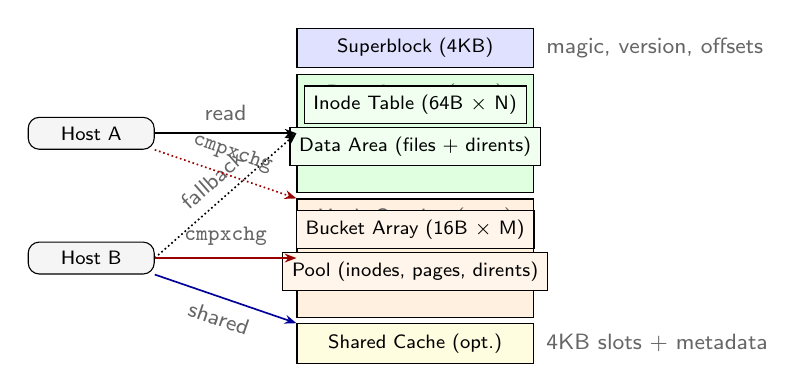
\begin{tikzpicture}[
    region/.style={draw, minimum width=3.0cm, minimum height=0.5cm,
      font=\scriptsize\sffamily, align=center},
    sub/.style={draw, minimum width=2.4cm, minimum height=0.4cm,
      font=\scriptsize\sffamily, align=center},
    mount/.style={draw, rounded corners, minimum width=1.6cm,
      minimum height=0.4cm, font=\scriptsize\sffamily, fill=gray!8},
    arr/.style={-{Stealth[length=1.5mm]}, semithick},
    note/.style={font=\footnotesize\sffamily, text=black!60},
  ]
  % --- DAX memory layout (center column) ---
  \node[region, fill=blue!12] (sb) at (0, 0) {Superblock (4KB)};
  \node[note, right=1pt of sb.east, anchor=west] {magic, version, offsets};

  % Base image with internal structure
  \node[region, fill=green!12, below=2pt of sb,
    minimum height=1.5cm] (base) {};
  \node[note, anchor=north] at (base.north) {Base Image (opt.)};
  \node[sub, fill=green!6, below=0.15cm of base.north] (itable)
    {Inode Table (64B $\times$ N)};
  \node[sub, fill=green!6, below=1pt of itable] (darea)
    {Data Area (files + dirents)};

  % Hash overlay
  \node[region, fill=orange!12, below=2pt of base,
    minimum height=1.5cm] (ovl) {};
  \node[note, anchor=north] at (ovl.north) {Hash Overlay (opt.)};
  \node[sub, fill=orange!8, below=0.15cm of ovl.north] (buckets)
    {Bucket Array (16B $\times$ M)};
  \node[sub, fill=orange!8, below=1pt of buckets] (pool)
    {Pool (inodes, pages, dirents)};

  % Page cache
  \node[region, fill=yellow!12, below=2pt of ovl] (pc)
    {Shared Cache (opt.)};
  \node[note, right=1pt of pc.east, anchor=west] {4KB slots + metadata};

  % --- Hosts (left column) ---
  \node[mount, left=1.8cm of base] (h1) {Host A};
  \node[mount, left=1.8cm of ovl] (h2) {Host B};

  % Both hosts read base image
  \draw[arr] (h1.east) -- (base.west)
    node[note, midway, above=1pt] {read};
  \draw[arr, densely dotted] (h2.east) -- (base.west)
    node[note, midway, above=1pt, sloped] {fallback};

  % Both hosts write through overlay
  \draw[arr, red!60!black] (h2.east) -- (ovl.west)
    node[note, midway, above=1pt] {\texttt{cmpxchg}};
  \draw[arr, red!60!black, densely dotted] (h1.south east) -- (ovl.north west)
    node[note, midway, above=1pt, sloped] {\texttt{cmpxchg}};

  % Both share pcache
  \draw[arr, blue!60!black] (h2.south east) -- (pc.north west)
    node[note, midway, below=1pt, sloped] {shared};

\end{tikzpicture}%
}
\caption{\daxfs memory layout on a shared memory region.
  Multiple OS instances access the same region concurrently: reads
  resolve from the overlay down to the base image; writes insert via
  \texttt{cmpxchg}; the shared cache serves all instances in the
  backing-store regime.}
\label{fig:arch}
\end{figure}

Figure~\ref{fig:arch} illustrates the layout.  The four regions shown
there, the superblock, the optional base image, the optional hash
overlay, and the optional shared cache, are laid out sequentially, and
the filesystem supports three modes depending on which are present.
In \emph{static mode}, only the superblock and base image are present,
and the image is self-contained and read-only.  \emph{Split mode} adds
the overlay and the shared cache, with bulk file data in a separate
backing file; this is the backing-store regime.  \emph{Empty mode} has
no base image, and all content is written through the overlay.

\subsection{On-Memory Format}
\label{sec:format}

\daxfs uses a deliberately simple flat format designed for safe
handling of untrusted images and efficient direct access.  There is no
disk: the four regions (superblock, base image, hash overlay, and
shared cache) are laid out sequentially in the shared memory region,
and each uses a 4\,KB header with magic numbers and size fields for
independent validation.

\subsubsection{Flat Directory Format}

Directories store fixed-size entries of 271 bytes each (the
\texttt{daxfs\_dirent} structure), containing a name length, an inode
number, a parent inode number, and a 254-byte inline name.  Unlike
pointer-based directory formats (htree in ext4, B-tree in Btrfs),
flat arrays have no cycles or dangling pointers, support bounded
iteration with a known upper bound, and can be fully validated in a
single sequential pass at mount time.

\subsubsection{Overlay Pool Entries}

Pool entries are variable-size.  \emph{Inode entries} (32\,B) store
mode, uid, gid, size, and timestamps, identified by a type header at
offset~0.  \emph{Data pages} (4\,KB) are raw file data with no
header; the entry type is inferred from the hash key encoding
(\S\ref{sec:overlay}).  Removing the header makes consecutively
allocated data pages contiguous in memory, enabling the read path to
coalesce sequential pages into a single large copy
(\S\ref{sec:zero-copy}).  \emph{Dirent entries} ($\sim$280\,B) record
the parent inode, name, target inode, mode, and a tombstone flag for
deletions.  \emph{Dirlist entries} (16\,B) serve as per-directory list
heads linking overlay dirents.

Each entry type has a per-type free list for recycling.  The free list
head is stored in the overlay header and updated via \texttt{cmpxchg},
making recycling lock-free across hosts.  Free-list recycling reuses
the first 8~bytes of the freed entry as the next-free pointer; for
data pages, these bytes are simply overwritten with user data on
reallocation.

\subsection{Zero-Copy Read Path}
\label{sec:zero-copy}

In \daxfs, file reads resolve to direct pointers into DAX memory
without any intermediate copying.  The read path first looks up the
data page in the hash overlay for key
\texttt{(ino $\ll$ 20) | pgoff}; if found, it returns a pointer
directly into the pool.  If absent, the path falls back to the base
image's data area using the inode's stored data offset.  For split
mode with a backing file, the path consults the shared page cache as a
final fallback.  At no point is data copied.  For \texttt{mmap}, the filesystem
installs PFN (page frame number) mappings directly to the DAX memory,
so user-space loads resolve to the physical memory in a single page
table walk.  Data pages are page-aligned in the pool, ensuring that
PFN mappings are always valid.

\subsection{Hash Overlay: Lock-Free Writes via CAS}
\label{sec:overlay}

The hash overlay is the core mechanism that enables concurrent
multi-host writes.  It is an open-addressing hash table with linear
probing, stored entirely in DAX memory, where all mutations use a
single 64-bit \texttt{cmpxchg}.

\subsubsection{Bucket Structure}

Each bucket is 16 bytes:

\begin{lstlisting}
struct daxfs_ovl_bucket {
  uint64_t state_key; /* bit 0: USED/FREE
                         bits 63:1: key    */
  uint64_t pool_off;  /* offset into pool  */
};
\end{lstlisting}

Bit~0 of \texttt{state\_key} distinguishes FREE (0) from USED (1).
The remaining 63 bits encode the lookup key.

\subsubsection{Key Encoding}

\daxfs encodes four entry types into the 63-bit key space:

\begin{itemize}
\item \textbf{Data page}: \texttt{(ino $\ll$ 20) | pgoff}.  Supports
  up to $2^{20}$ pages (4\,GB) per file.
\item \textbf{Inode metadata}: \texttt{(ino $\ll$ 20) | 0xFFFFF}.
  The sentinel page offset distinguishes inode entries from data.
\item \textbf{Directory list head}: \texttt{(ino $\ll$ 20) | 0xFFFFE}.
  Points to the first overlay dirent for a directory.
\item \textbf{Directory entry}: \texttt{FNV-1a(parent\_ino, name)}.
  A 63-bit hash of the parent inode number and entry name.
\end{itemize}

\subsubsection{Insert Protocol}

To insert a new entry, a host:
\begin{enumerate}
\item Computes \texttt{hash = key \% bucket\_count}.
\item Reads \texttt{bucket[hash].state\_key}.
\item If FREE: attempts \texttt{cmpxchg(\&bucket[hash].state\_key, 0,
  key $\ll$ 1 | 1)}.  On success, allocates a pool entry and writes
  \texttt{pool\_off} with \texttt{smp\_wmb} ordering.  On failure
  (another host won the race), retries from step~2.
\item If USED with matching key: the entry already exists (update or
  conflict).
\item If USED with different key: linear probe to \texttt{hash+1} and
  repeat.
\end{enumerate}

This protocol is lock-free: no instance can block another.  Hash
collisions are resolved by linear probing.  We use open addressing with
linear probing rather than chaining or cuckoo hashing for two reasons.
First, it keeps every entry inside the contiguous, bump-allocated pool
with no cross-instance pointers to chase, which lets a single
sequential pass validate the whole image at mount time and avoids
pointer-cycle attacks on untrusted images.  Second, linear probing
touches consecutive cache lines, suiting the load-store access pattern
of shared memory.  The overlay is sized for a load factor below 70\%,
where the average probe length is under three; \daxfs does not resize
online, because resizing would require a stop-the-world migration
coordinated across all instances (\S\ref{sec:discussion}).

\subsubsection{Pool Allocator}

Pool entries are variable-size: inodes (32\,B), data pages
(4\,KB), and dirents ($\sim$280\,B).  Allocation uses an
atomic bump pointer with type-dependent alignment:

\begin{lstlisting}
aligned = ALIGN(pool_alloc, align);
off = atomic_cmpxchg(&hdr->pool_alloc,
                     pool_alloc,
                     aligned + size);
\end{lstlisting}

Metadata entries use 8-byte alignment; data pages use \texttt{PAGE\_SIZE}
alignment.  Page-aligning data allocations serves two purposes:
(1)~it enables DAX \texttt{mmap} to install PFN mappings directly to
overlay pages, and (2)~it ensures that consecutive data page allocations
produce contiguous memory, enabling read-path coalescing
(\S\ref{sec:zero-copy}).  The alignment gap between a metadata entry
and the next data page is at most 4\,KB of wasted pool space, a
negligible fraction of typical pool sizes (64\,MB+).

Freed entries are recycled through per-type lock-free free lists (CAS
on list head), avoiding pool exhaustion for long-running workloads.

\subsubsection{Directory Operations}

Each directory maintains a per-directory linked list of overlay
dirents.  The list head is stored at key
\texttt{(dir\_ino $\ll$ 20) | 0xFFFFE}.  \texttt{readdir} iterates
both the base image dirent array and the overlay list, with overlay
entries taking precedence.  Deletion uses tombstone entries.

\subsection{Shared Cache and MH-Clock}
\label{sec:pcache}

The shared cache (\emph{pcache}) serves the backing-store regime: when
a dataset is larger than the shared memory region, its bulk data lives
in a backing file and the cache holds the hot pages.  Crucially, the
cache itself resides in shared memory, so a single cached copy is
directly accessible to every instance, in contrast to a per-instance
kernel page cache that would hold $N$ copies.  The cache is the only
part of \daxfs that requires coordinated eviction across instances, and
the algorithm that performs it, MH-clock, is described in
\S\ref{sec:mhclock}.

\subsubsection{Slot State Machine}

Each cache slot has a 16-byte metadata entry:

\begin{lstlisting}
struct daxfs_pcache_slot {
  __le64 state_tag; /* bits[1:0]=state,
     bits[5:2]=refcount, bits[63:6]=tag */
  __le32 ref_bit;   /* clock: recently used */
  __le32 reserved;
};
\end{lstlisting}

The state machine uses three states encoded in the low 2 bits:

\begin{center}
\texttt{FREE (0) $\xrightarrow{\texttt{cmpxchg}}$ PENDING (1)
  $\xrightarrow{\texttt{cmpxchg}}$ VALID (2)}
\end{center}

Bits [5:2] hold a 4-bit refcount (0--15 concurrent readers),
and the upper 58 bits encode the tag identifying which file page this
slot caches (\S\ref{sec:overlay}).  Packing state, refcount, and tag into a single 64-bit
word allows a single \texttt{cmpxchg} to atomically update all three
fields, which is essential for lock-free multi-host coordination.

\textbf{Fill protocol.}  When a host needs a page not in the cache:
\begin{enumerate}
\item Probe up to 8 slots starting at the hash position.  The window of
  8 bounds the work of a lookup and spans two 64-byte cache lines of
  slot metadata, so a full probe touches at most two lines; \daxfs
  sizes the cache for a load factor at which 8 slots almost always hold
  a match or a free slot.  If a matching VALID slot is found, pin it
  (CAS-increment refcount) and return.  If a FREE slot is found, record
  it.
\item \texttt{cmpxchg} the FREE slot from FREE to PENDING with the
  desired tag.  If another host wins, retry.
\item Read the backing file page into the slot's data area via
  \texttt{kernel\_read}.
\item \texttt{cmpxchg} the slot from PENDING to VALID.
\end{enumerate}

Other hosts that need the same page during step~3 see the PENDING
state and busy-poll until VALID, avoiding duplicate reads from the
backing file.

\subsubsection{Decentralized Eviction: MH-Clock}
\label{sec:mhclock}

Eviction is the one place where independent instances must agree on
which slot to reclaim, and it is where standard cache algorithms break
down: CLOCK, LRU, and their variants all assume a single coordinator,
namely one OS holding one clock hand or one lock.  None can run
unmodified across instances that share a cache with no central
authority.  MH-clock, to our knowledge the first decentralized,
lock-free adaptation of CLOCK for a shared multi-instance cache,
removes that assumption.  Adapted from the classic CLOCK
algorithm~\cite{corbato68:clock}, it has no central hand: each instance
independently selects victims within its local probe window using three
escalating phases:

\begin{enumerate}
\item \textbf{Cold victim.}  Scan the 8-slot probe window for a
  VALID slot with \texttt{ref\_bit}=0 and refcount=0.  If found,
  CAS it to FREE and restart the fill.
\item \textbf{Clear and yield.}  If all probed slots are hot
  (\texttt{ref\_bit}=1), clear their \texttt{ref\_bit} fields and
  yield the CPU briefly (\texttt{cpu\_relax}).  This gives other
  hosts an opportunity to re-touch genuinely hot entries before
  the re-scan.
\item \textbf{Re-scan.}  Scan again for a cold, unpinned victim.
  If still none, force-evict the first VALID slot with refcount=0,
  ignoring \texttt{ref\_bit}.
\end{enumerate}

A separate background clock sweep periodically advances a shared
atomic \texttt{evict\_hand} counter by 64 slots using
\texttt{cmpxchg}; the host that wins the CAS clears
\texttt{ref\_bit} on all VALID slots in that window.  Hosts that
lose the race skip the sweep, ensuring that only one host clears
each window and \texttt{ref\_bit} values decay at a controlled rate even under
contention.

The refcount in \texttt{state\_tag} ensures that slots actively
being read by any host are never evicted.  Readers CAS-increment
the refcount before accessing slot data and CAS-decrement it
afterward, providing safe pinning without locks.

\subsubsection{Multi-File Support}

The tag encoding \texttt{(ino $\ll$ 20) | pgoff} supports up to
$2^{20}$ pages (4\,GB) per file.  Multiple backing files share the
same cache through a backing file array in the superblock, with inode
numbers namespaced per file.

\subsection{Cross-Instance Coherency}
\label{sec:coherency}

Recall the two-tier model of \S\ref{sec:coherence-assume}: coordination
structures use \texttt{cmpxchg} and need hardware-coherent atomics,
while bulk data needs only ordered visibility.  Two mechanisms
implement the data tier:

\paragraph{File-size coherency.}
When one instance appends data and updates the file size in the overlay
inode entry, another instance must see the new size.  \daxfs stores the
authoritative \texttt{i\_size} in the overlay inode entry in shared
memory.  On each read-path entry, \daxfs performs a \texttt{READ\_ONCE}
on the overlay's size field and updates the in-kernel VFS inode, so
reads always see the latest file size without explicit invalidation
messages.

\paragraph{Memory ordering.}
Insert operations use \texttt{smp\_wmb} between writing pool entry
contents and writing the bucket's \texttt{pool\_off} field.
Lookup operations use \texttt{smp\_rmb} after reading
\texttt{pool\_off} to ensure they see the complete pool entry.
On x86, these compile to compiler barriers (x86 provides TSO
ordering); on ARM64, they emit fence instructions.

%-------------------------------------------------------------------------------
\section{Implementation}
\label{sec:impl}
%-------------------------------------------------------------------------------

\daxfs is implemented as a loadable Linux kernel module in
approximately 2,500 lines of C.  It registers a filesystem type
(\texttt{daxfs}) and supports both the legacy \texttt{mount(2)}
interface and the modern \texttt{fsopen}/\texttt{fsconfig}/\texttt{fsmount}
interface introduced in Linux~5.6.

\subsection{Memory Mapping}

\daxfs supports two memory backing modes.  In the \emph{physical
address} path, the \texttt{phys=} and \texttt{size=} mount options
cause \daxfs to call \texttt{memremap()} on the specified physical
range; this is the primary path for Optane PMem and CXL memory
devices.  Alternatively, the \emph{DMA buffer} path uses the
\texttt{fsopen} API: a user-space process passes a dma-buf file
descriptor via \texttt{FSCONFIG\_SET\_FD}, and \daxfs calls
\texttt{dma\_buf\_vmap()} to obtain a kernel virtual mapping.  Both
modes bypass the kernel's \texttt{dax\_device} abstraction entirely,
mapping memory directly into the filesystem's address space.

\subsection{VFS Integration}

\daxfs registers standard VFS operations.  Inode operations (lookup,
create, mkdir, symlink, rename, unlink, setattr) all route writes
through the hash overlay; the base image is never modified.

The \texttt{read\_iter} file operation performs zero-copy reads by
returning pointers into DAX memory.  For overlay data, the read path
detects physically contiguous pages and coalesces them into a single
\texttt{copy\_to\_iter} call: because data pages are raw 4\,KB
allocations with no header, pages allocated by the same bump operation
are adjacent in memory.  After looking up the first page (via the
per-inode xarray cache), the read path checks whether subsequent pages
are physically adjacent and, if so, extends the copy region.  For a
16\,MB sequential read of sequentially written data, this reduces the
operation from 4,096 individual copies to a single contiguous transfer.
For pcache-backed data, the read path pins the cache slot (incrementing
refcount) before returning data, preventing eviction during the read.
Address space operations (\texttt{readpage}/\texttt{readahead}) provide
integration with the kernel page cache on non-DAX access paths.

Data resolution on every read path calls
\texttt{daxfs\_refresh\_isize()}, which performs a \texttt{READ\_ONCE}
on the overlay's size field, ensuring cross-host coherency of file
sizes without explicit invalidation.

\subsection{Mount-Time Validation}

The flat format (\S\ref{sec:format}) enables complete image validation
in a single sequential scan at mount time.  When the \texttt{validate}
option is specified, \daxfs checks superblock integrity, inode table
bounds, directory entry references, and region overlap.  The absence
of pointer-based structures eliminates cycle injection, dangling
pointer exploitation, and unbounded traversal, which is important for
mounting untrusted images in container environments.

\subsection{Multikernel Deployment}
\label{sec:multikernel-impl}

\daxfs runs unmodified across multiple kernels.  Each kernel mounts the
same shared physical window through the \texttt{phys=} path: the window
is reserved outside every kernel's private RAM and mapped with
\texttt{memremap(MEMREMAP\_WB)}, the same code path used for a CXL
physical-address device.  No cross-kernel mechanism beyond this is
required, because an x86 \texttt{LOCK CMPXCHG} on a shared address is
globally atomic across all cores in the coherence domain regardless of
which kernel issued it~\cite{intel:sdm}.  The number of kernels mapping
the region is the only difference between the multikernel deployment
and a CXL multi-host deployment.

%-------------------------------------------------------------------------------
\section{Evaluation}
\label{sec:evaluation}
%-------------------------------------------------------------------------------

We evaluate \daxfs against the question each part of the motivation
raised.  \S\ref{sec:eval-memory} measures the memory footprint of
sharing one base image across instances, the headline of
\S\ref{sec:motivation}; \S\ref{sec:eval-correct} establishes
cross-kernel correctness on real hardware; \S\ref{sec:eval-write}
measures concurrent write scaling; \S\ref{sec:eval-cache} evaluates the
shared cache and MH-clock; \S\ref{sec:eval-overhead} isolates
single-instance mechanism overhead; and \S\ref{sec:eval-cxl}
characterizes the CXL generalization by emulation.

\subsection{Experimental Setup}

\textbf{Multikernel testbed (primary).}  We partition a single server
into up to four independent Linux kernels on disjoint cores.  A
physical memory window is reserved outside every kernel's private RAM
and mapped into each kernel through the \texttt{phys=} path
(\S\ref{sec:multikernel-impl}); all kernels mount the same \daxfs image
over this window.  Because the kernels share one hardware coherence
domain, a \texttt{cmpxchg} issued by any kernel is genuinely atomic
with respect to the others, with no emulation.
\todo{exact CPU, core and memory partitioning, shared window size}

\textbf{Single-instance platform.}  \todo{CPU, DRAM.}  A DRAM-backed
region mapped via \texttt{memremap(MEMREMAP\_WB)} exercises the same
write-back-cached path a CXL device uses.  We use it to isolate
single-instance overhead at thread counts up to the full core count.

\textbf{CXL emulation.}  To characterize the latency of the CXL
generalization, we use a QEMU setup in which two virtual hosts share a
memory region and CXL atomic requests are forwarded between them
(\S\ref{sec:eval-cxl}).  This measures fabric latency only; all
correctness and scaling results use the real multikernel testbed.

\textbf{Baselines.}  FamFS~\cite{groves24:Famfs}, the closest
shared-memory filesystem; EROFS~\cite{gao20:erofs}, a read-only image
format with a per-kernel cache; and tmpfs, the in-memory performance
ceiling.  \todo{confirm versions and configurations}

\textbf{Workloads.}  \todo{container base image(s) and sizes; fio
configuration; number of runs and the statistic reported.}

\subsection{Memory Footprint}
\label{sec:eval-memory}

This is the result the motivation demands: running $N$ instances from a
shared base image should cost one copy, not $N$.  We boot one to four
kernels, each running a container from the same base image, and measure
the total physical memory attributable to the filesystem and its cache.
Under EROFS and tmpfs, total memory grows roughly linearly with the
number of instances, because each instance holds its own copy of the
image and its own cache.  Under \daxfs, the shared base image and the
shared cache are counted once, and only the per-instance writable
overlay grows with $N$.  We report both the DAX-resident regime, where
the image fits in shared memory, and the backing-store regime, where a
larger-than-memory dataset is served through the shared cache.

\todo{Figure: total filesystem memory vs.\ number of instances (1--4),
\daxfs vs.\ EROFS vs.\ tmpfs, for both regimes.}
\todo{E1 numbers: per-instance and aggregate footprint; the linear
($N\!\times\!S$) versus constant-plus-delta ($S + N\delta$) comparison.}

\subsection{Cross-Kernel Correctness}
\label{sec:eval-correct}

\daxfs's coordination must stay correct when independent kernels mutate
shared structures at once.  On the multikernel testbed we drive all
four kernels to insert and update overlay entries that collide on the
same buckets, and to fill and evict the same cache slots, then check
for lost updates and torn reads.

\todo{Figure: CAS success rate and lost-update count vs.\ number of
kernels under forced contention.}
\todo{E2 numbers: CAS accuracy, zero lost updates, retry rate.}  Unlike
the earlier QEMU result (\S\ref{sec:eval-cxl}), these come from real
hardware atomics across real kernels, which is the evidence the prior
version of this work lacked.

\subsection{Concurrent Write Scaling}
\label{sec:eval-write}

A shared filesystem is useful only if concurrent writers do not
serialize.  We measure aggregate write throughput as the number of
writing kernels grows from one to four, each writing into its own
overlay.  FamFS cannot run this experiment: its clients cannot create,
append, or delete, so only the single master writes.  That contrast is
the point, since lock-free concurrent writes from every instance are
exactly what \daxfs adds over the closest prior system.

\todo{Figure: aggregate write throughput vs.\ number of writing
kernels, \daxfs vs.\ the FamFS single-writer ceiling.}
\todo{E3 numbers: scaling from 1 to 4 kernels.}

\subsection{Shared Cache and MH-Clock}
\label{sec:eval-cache}

In the backing-store regime the shared cache must keep a high hit rate,
scale as instances are added, and treat instances fairly, all with no
central eviction coordinator.  We sweep the working-set-to-cache-size
ratio and measure hit rate; we vary the number of kernels and measure
aggregate cache throughput; and we measure each kernel's share of cache
residency under a balanced load.

We do not compare MH-clock against simpler heuristics such as random or
FIFO, because its contribution is not a better heuristic but a
decentralized one: standard CLOCK, LRU, and their variants assume a
single coordinator and cannot run unmodified across instances sharing a
cache (\S\ref{sec:mhclock}).  The relevant alternatives are a
per-instance cache, which EROFS embodies and which
\S\ref{sec:eval-memory} shows sacrifices the memory saving, and a
centrally locked cache, which serializes the very scaling measured
here.

\todo{Figure: hit rate vs.\ working-set/cache ratio (miss rate must
rise as the working set exceeds the cache); aggregate throughput and
per-kernel fairness vs.\ number of kernels.}
\todo{E4 numbers: hit rate across the sweep, scaling to 4 kernels,
fairness index.  The prior hit-rate measurement contained a bug and is
being re-run.}

\subsection{Single-Instance Overhead}
\label{sec:eval-overhead}

The lock-free mechanism should add little overhead on a single
instance, where there is no contention to win.  On the single-instance
platform we compare \daxfs against tmpfs and ext4-dax on sequential and
random fio workloads, scaling threads to the full core count.
Figures~\ref{fig:read-throughput}--\ref{fig:summary} report preliminary
single-instance results.  \todo{re-run on the new configuration and to
the full thread count (E5 numbers); the figures below are placeholders
from the prior measurement.}

\begin{figure}[t]
\centering
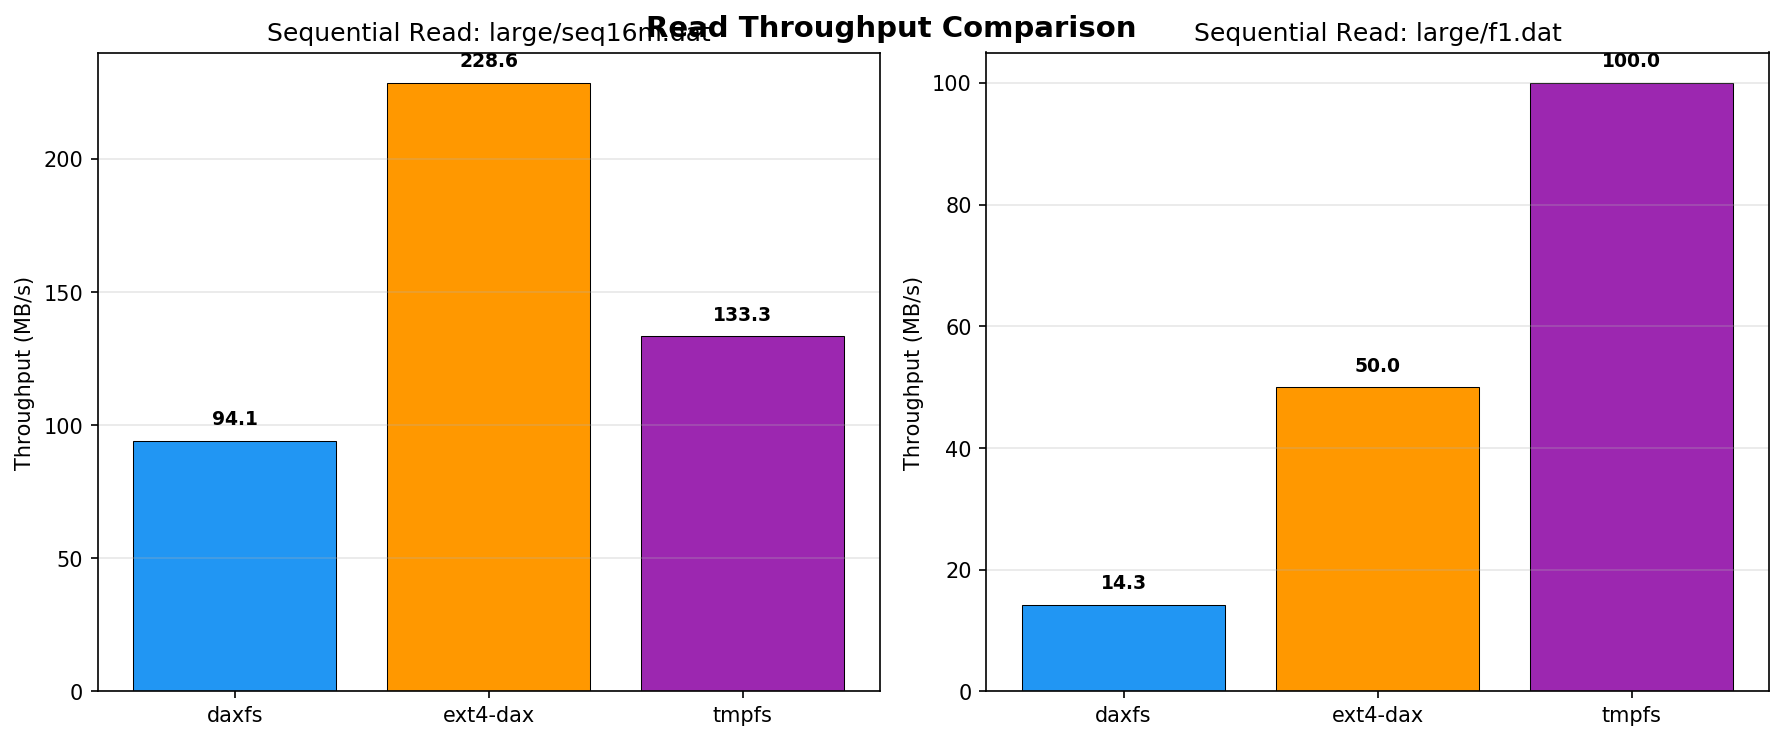
\includegraphics[width=\columnwidth]{read_throughput.png}
\caption{Sequential read throughput comparison across filesystems
  (Intel Xeon Gold 5418Y, DRAM-backed DAX).
  Left: 16\,MB sequential read; right: 1\,MB sequential read.
  \daxfs achieves 59.2\,MB/s on the large sequential workload
  (6.2$\times$ ext4-dax) and matches tmpfs on the 1\,MB file
  (100\,MB/s each).  The 16\,MB gap versus tmpfs (228.6\,MB/s)
  reflects the overhead of per-page overlay resolution on large
  sequential scans; at 1\,MB the overhead is amortized.}
\label{fig:read-throughput}
\end{figure}

\begin{figure}[t]
\centering
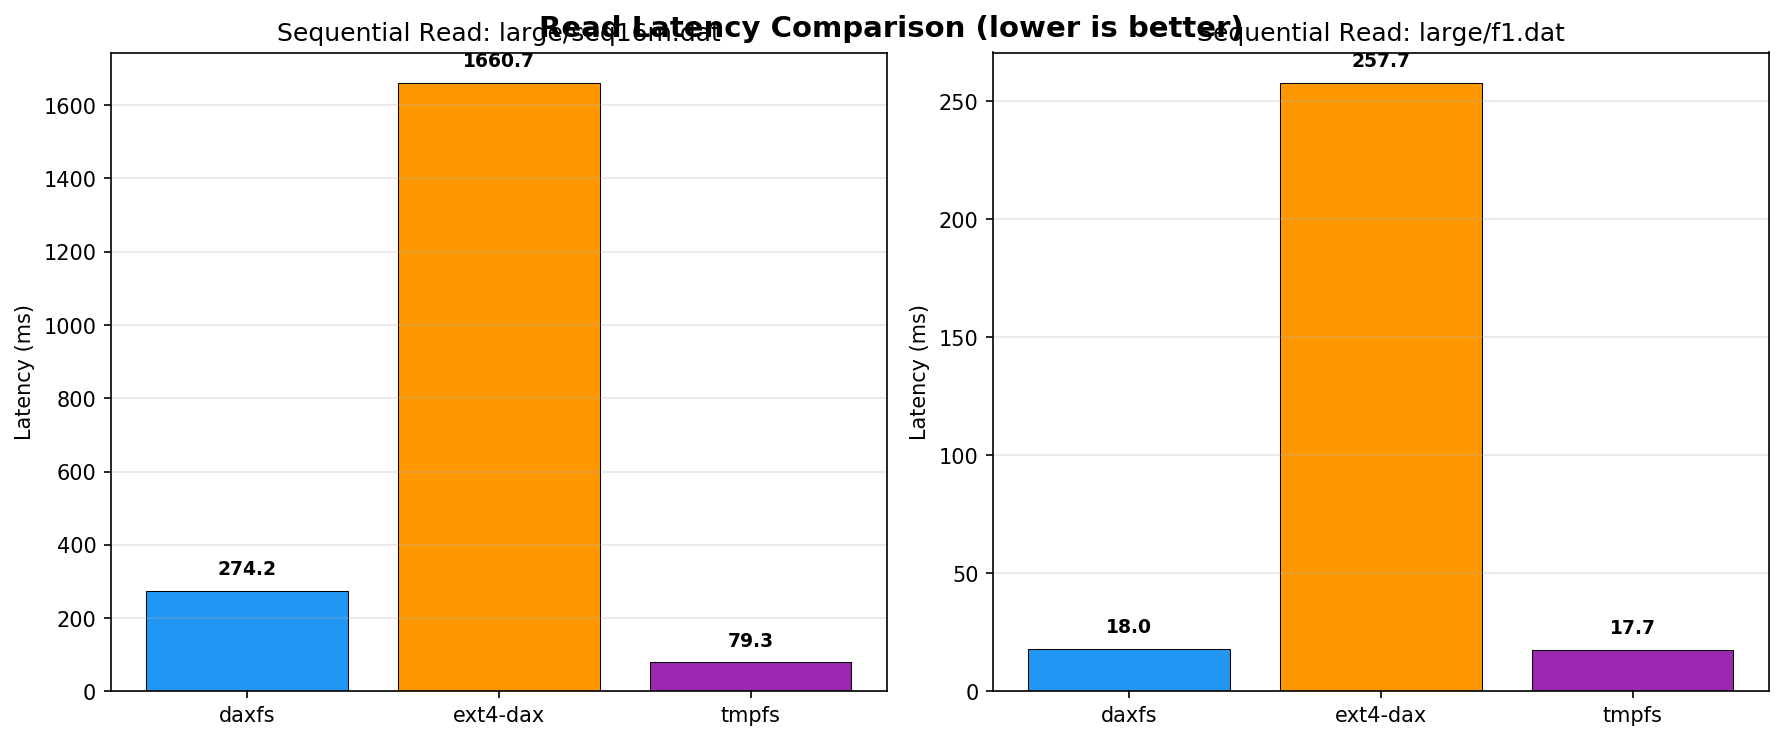
\includegraphics[width=\columnwidth]{read_latency.png}
\caption{Sequential read latency comparison (lower is better).
  \daxfs completes a 16\,MB read in 274.2\,ms, 6.1$\times$ faster
  than ext4-dax (1,660.7\,ms).  On 1\,MB files, \daxfs and tmpfs
  finish in 18.0 and 17.7\,ms respectively.}
\label{fig:read-latency}
\end{figure}

\begin{figure}[t]
\centering
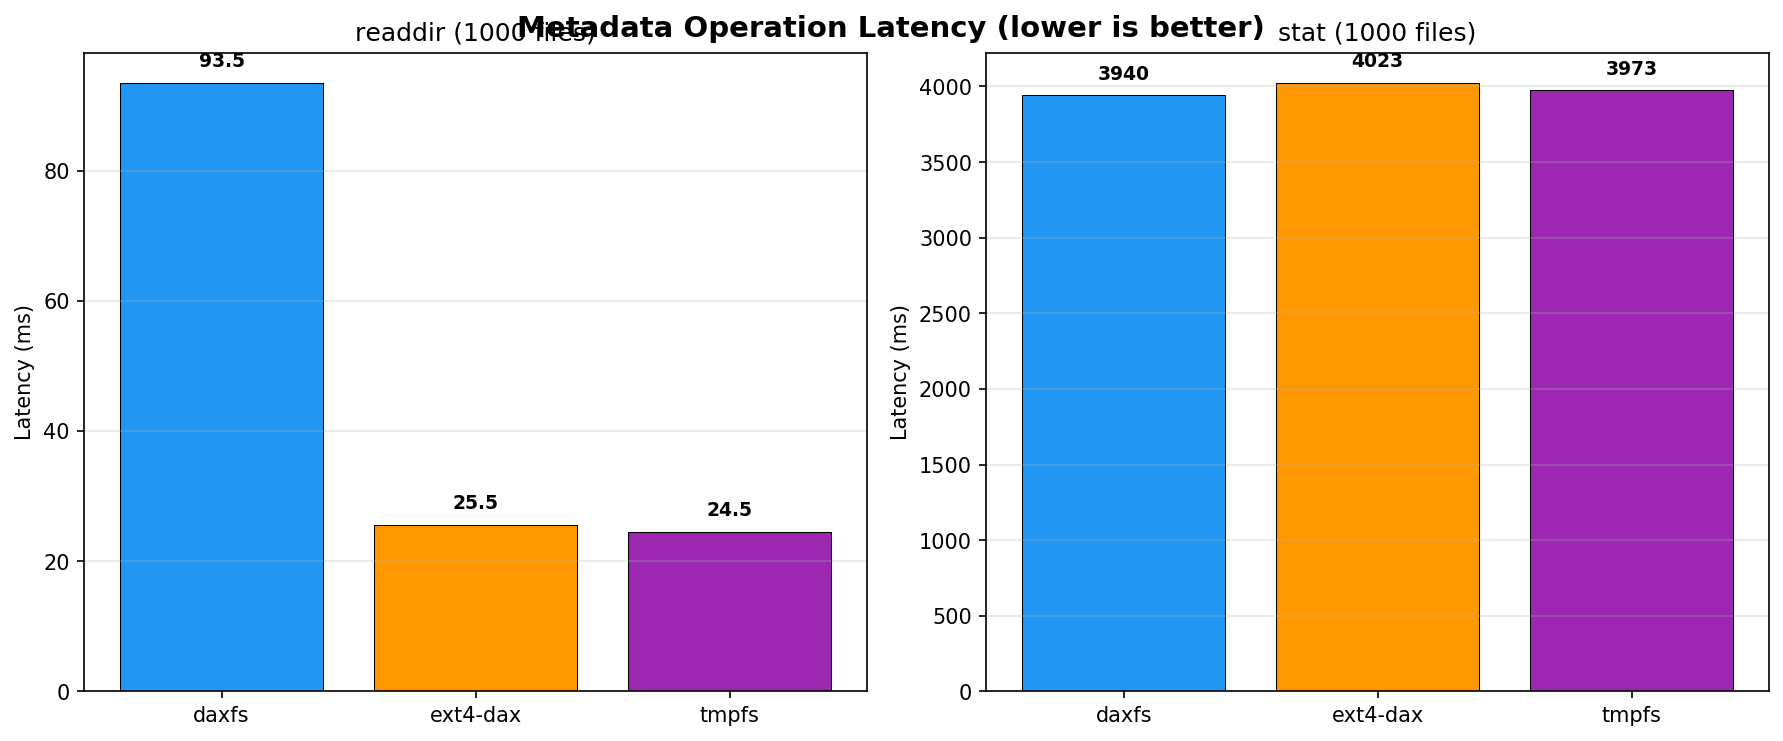
\includegraphics[width=\columnwidth]{metadata.png}
\caption{Metadata operation latency on 1,000 files (lower is better).
  \daxfs achieves the lowest \texttt{stat} latency (3,528\,ms),
  4.6\% faster than ext4-dax (3,699\,ms) and 6.3\% faster than tmpfs
  (3,764\,ms), due to flat overlay lookup.  On \texttt{readdir},
  \daxfs (33.8\,ms) is slower than tmpfs (23.1\,ms) and ext4-dax
  (23.9\,ms) due to the cost of iterating both the base image dirent
  array and the overlay linked list.}
\label{fig:metadata}
\end{figure}

\begin{figure}[t]
\centering
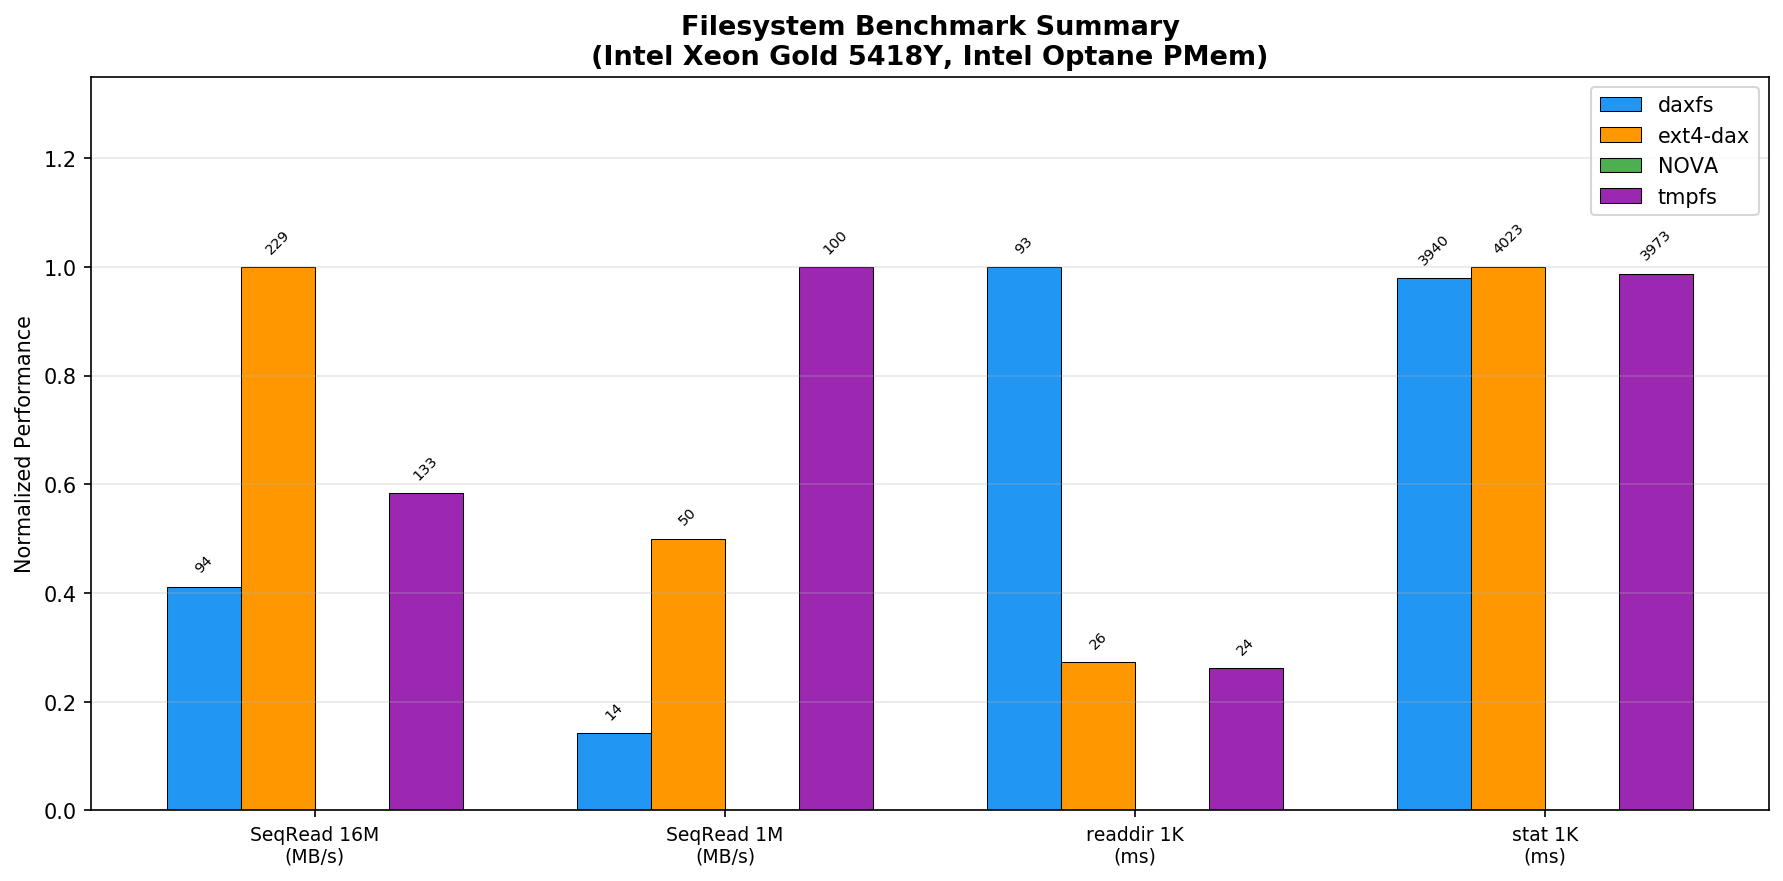
\includegraphics[width=\columnwidth]{summary.png}
\caption{Normalised performance summary across all benchmarks
  (Intel Xeon Gold 5418Y, DRAM-backed DAX).  Each group is
  normalised to the best-performing filesystem.  \daxfs matches
  tmpfs on 1\,MB sequential reads and achieves the lowest
  \texttt{stat} latency, while outperforming ext4-dax on data I/O.
  The 16\,MB sequential read and \texttt{readdir} gaps versus tmpfs
  reflect per-page overlay lookup and dual-source directory iteration
  overhead.}
\label{fig:summary}
\end{figure}

\subsection{CXL Generalization}
\label{sec:eval-cxl}

The multikernel testbed shares memory within one machine; CXL~3.0
extends the same \texttt{cmpxchg} coordination across machines, at
higher latency.  To characterize that latency we use a QEMU setup in
which two virtual hosts share a memory region and CXL atomic requests
are forwarded between them.  This is an emulation of fabric latency, not
a correctness experiment; correctness is established on real hardware
in \S\ref{sec:eval-correct}.

In the emulation, cross-host atomics run far slower than local DRAM
atomics, a gap dominated by the forwarding cost rather than by \daxfs,
and batching amortizes the per-operation cost
(Figure~\ref{fig:multihost}).  Hardware CXL~3.0 switches are expected to
bring cross-host atomic latency into the microsecond range, which would
narrow this gap substantially.  \todo{update the emulation numbers and
reframe the figure as fabric-latency characterization only.}

\begin{figure}[t]
\centering
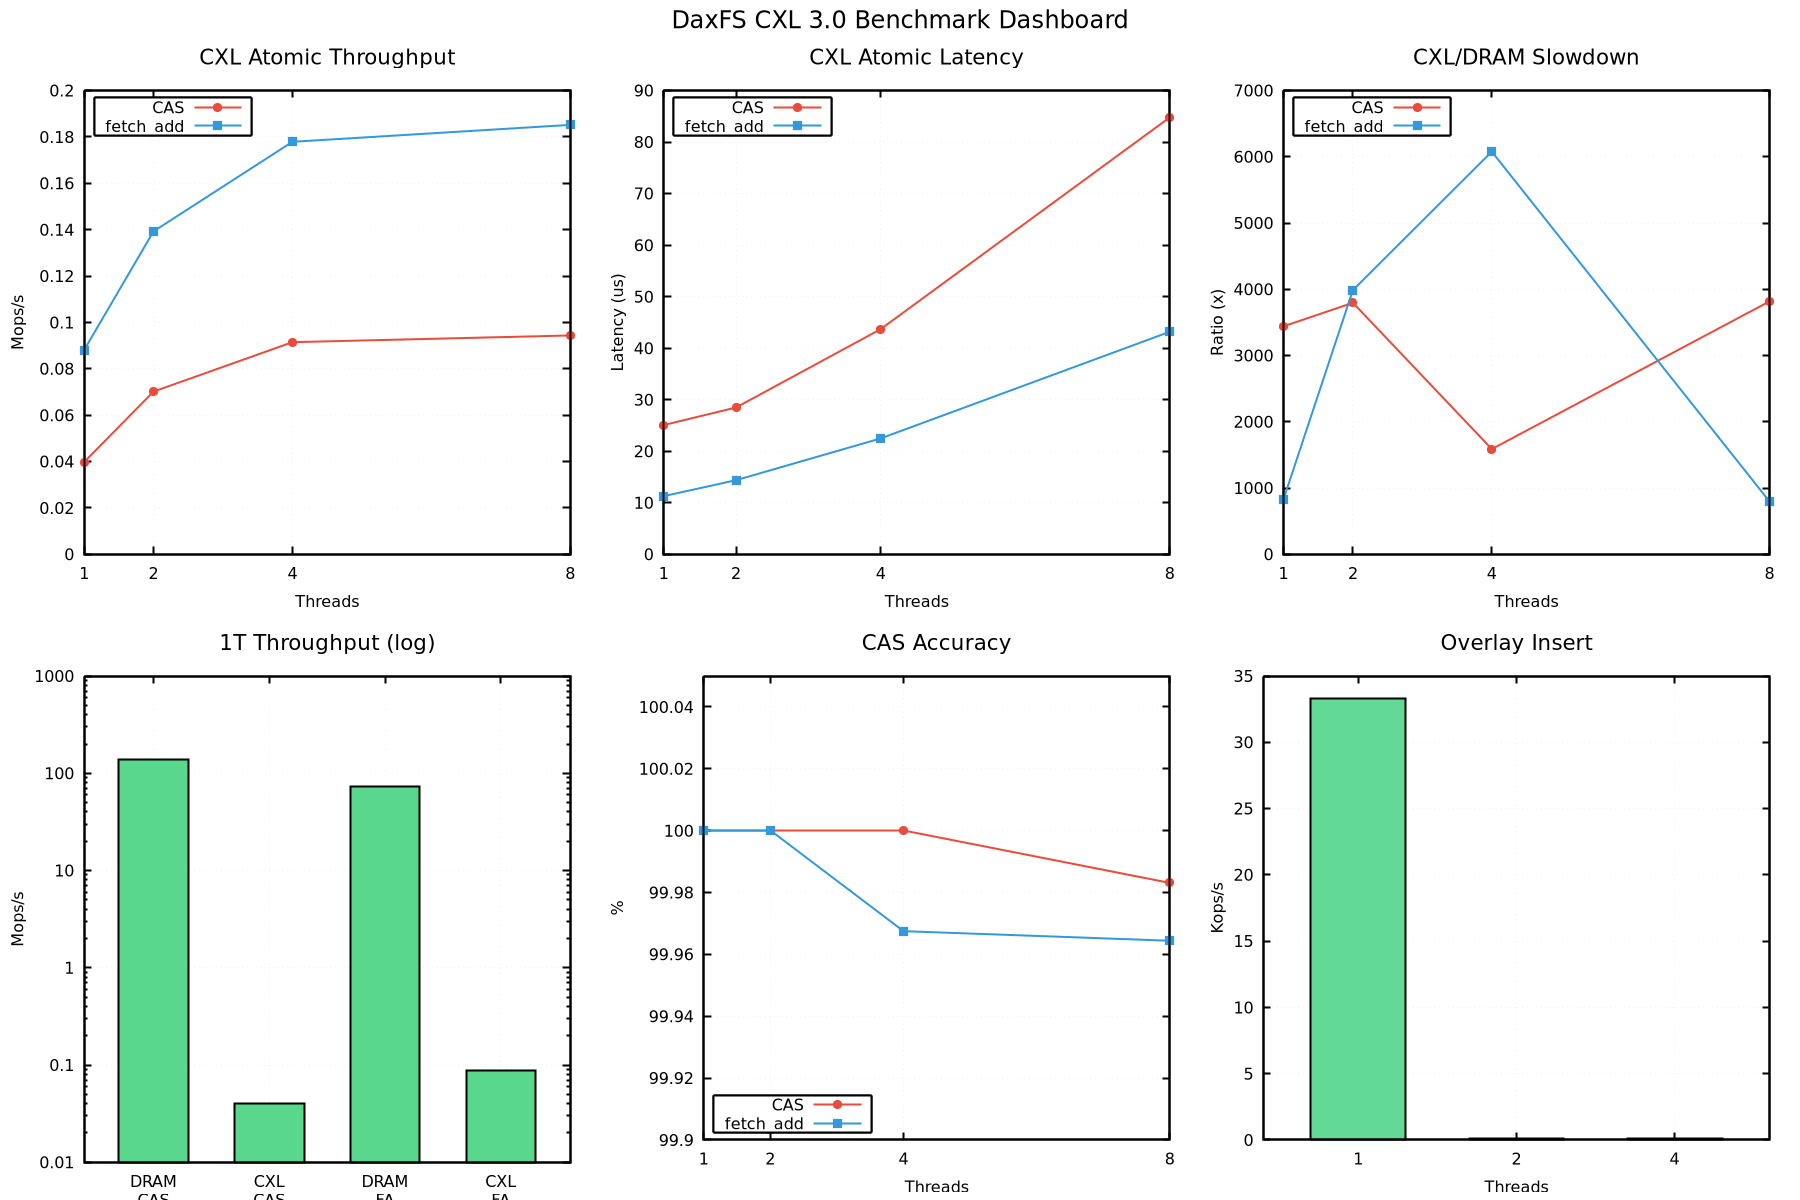
\includegraphics[width=\columnwidth]{fig6_dashboard.png}
\caption{CXL fabric-latency characterization (QEMU emulation, two
  virtual hosts, TCP-forwarded atomics).  This emulation bounds the
  latency of the CXL generalization only; all correctness and scaling
  results use the real multikernel testbed (\S\ref{sec:eval-correct}).
  \todo{regenerate without the CAS-accuracy panel, which is now
  measured on real hardware in \S\ref{sec:eval-correct}.}}
\label{fig:multihost}
\end{figure}

%-------------------------------------------------------------------------------
\section{Related Work}
\label{sec:related}
%-------------------------------------------------------------------------------

\paragraph{Persistent memory filesystems.}
PMFS~\cite{dulloor14:pmfs}, NOVA~\cite{xu16:nova},
Strata~\cite{kwon17:strata}, and SplitFS~\cite{kadekodi19:splitfs}
target single-host persistent memory.  All maintain complex metadata
structures (B-trees, per-inode logs) that cannot be shared across
hosts without distributed locking.  \daxfs replaces these with a flat
base image and lock-free hash overlay.

\paragraph{CXL shared memory systems.}
Pond~\cite{li23:pond} and TPP~\cite{maruf23:tpp} focus on CXL memory
management, not filesystem semantics.  FamFS~\cite{groves24:Famfs} is
architecturally the closest prior work to \daxfs.  Both provide a
filesystem interface to CXL shared memory, supporting multiple hosts
mounting the same DAX region.  However, FamFS uses a single-master
log-replay model: one designated host pre-allocates files and clients
replay its metadata log.  Clients cannot create, append, truncate, or
delete files, and there is no shared cache or CXL-atomic coordination
(see Table~\ref{tab:feature-matrix} for a feature comparison).

\paragraph{Distributed filesystems.}
GFS~\cite{ghemawat03:gfs}, CephFS~\cite{weil06:ceph},
Lustre~\cite{schwan03:lustre}, Orion~\cite{yang20:orion}, and
Assise~\cite{anderson20:assise} use message-passing or RPC, adding
$\mu$s-scale latency that shared memory makes unnecessary.

\paragraph{Multikernel operating systems.}
Barrelfish~\cite{baumann09:multikernel} and Popcorn
Linux~\cite{barbalace15:popcorn} run multiple OS instances on one
machine and coordinate through shared memory or message passing.  They
provide OS services, not a shared filesystem; \daxfs gives such
instances a shared, writable storage layer coordinated entirely by
hardware atomics.

\paragraph{Container image distribution and lock-free structures.}
EROFS~\cite{gao20:erofs} and Slacker~\cite{harter16:slacker} speed up
container start by distributing read-only images, but each instance
keeps its own copy and cache; neither shares one writable image across
instances.  \daxfs's overlay draws on lock-free hash table
designs~\cite{michael02:lockfree,herlihy08:art}, adding lock-free
free-list recycling via \texttt{cmpxchg}.

%-------------------------------------------------------------------------------
\section{Discussion}
\label{sec:discussion}
%-------------------------------------------------------------------------------

\daxfs makes deliberate choices that trade generality for a small,
validatable, lock-free core.  We discuss the main ones and where they
apply.

\paragraph{Sizing over resizing.}
The overlay and cache are sized at creation time and do not resize
online, because resizing would require a stop-the-world migration
across all instances.  Sizing the bucket count for a load factor below
70\% keeps the average probe length under three; it reaches 5.5 only at
90\% load.  For the container workload, where image sizes are known at
deployment, static sizing is a natural fit.

\paragraph{Flat directories.}
The flat directory format trades lookup asymptotics for validatability.
Lookup is $O(n)$ in directory size, competitive with indexed formats up
to roughly a thousand entries, and it is what lets the whole image be
checked in a single pass.  Very large directories would benefit from an
overlay index, which the format can accommodate.

\paragraph{Persistence.}
\daxfs relies on ADR or eADR for persistence and does not issue explicit
\texttt{clflush}/\texttt{clwb}; on platforms without ADR a crash could
lose recent overlay insertions.  Adding cache-line flushes is
straightforward and trades latency for durability, and the container
images we target are reconstructible.

\paragraph{Scope.}
\daxfs targets container and dataset sharing, so it omits features those
workloads do not use: \texttt{mknod}, extended attributes, online pool
compaction, and names beyond 255 characters.  Each is additive rather
than fundamental to the design.

\paragraph{Toward GPUs and CXL hardware.}
Because \daxfs coordinates entirely through \texttt{cmpxchg}, the same
primitive extends to accelerators that issue PCIe AtomicOps: a GPU could
read shared data through a \texttt{dma-buf} export and participate in
cache lookups without CPU mediation, an alternative to the block-layer
path of GPUDirect Storage~\cite{gpudirect:storage} and
BaM~\cite{bam23:gpussd}.  We leave GPU integration to future work.
Likewise, as CXL~3.0 switch hardware becomes available, the multikernel
results here should carry over to multi-host deployments with only the
fabric latency of \S\ref{sec:eval-cxl} added.

%-------------------------------------------------------------------------------
\section{Conclusion}
\label{sec:conclusion}
%-------------------------------------------------------------------------------

Multiple OS instances sharing physical memory, multikernels today and
CXL multi-host tomorrow, need a filesystem to share container images,
not a raw byte array.  \daxfs provides one using \texttt{cmpxchg} as its
sole coordination primitive, achieving lock-free concurrent writes,
base-plus-overlay sharing of a single writable image, and a cooperative
shared cache with decentralized MH-clock eviction, all with no locks,
logs, or central coordinator.

We evaluate \daxfs on real multikernel hardware, where it shares one
base image across instances instead of $N$ copies (\todo{E1}), sustains
correct lock-free cross-kernel coordination under contention
(\todo{E2}), and adds negligible single-instance overhead (\todo{E5}),
and we characterize the CXL generalization by emulation.  As CXL~3.0
hardware matures, the same design carries over to disaggregated memory
shared across hosts.

%-------------------------------------------------------------------------------
\section*{Availability}
%-------------------------------------------------------------------------------

\daxfs is available as open-source software~\cite{daxfs:repo}.  The
implementation includes the Linux kernel module, \texttt{mkdaxfs}
image creation tool, and \texttt{daxfs-inspect} debugging tool.

%-------------------------------------------------------------------------------
\begin{thebibliography}{26}

\bibitem{anderson20:assise}
T.~E. Anderson, M.~Canini, J.~Kim, D.~Kostic, Y.~Kwon, S.~Peter,
  W.~Pugh, and E.~Witchel.
\newblock Assise: Performance and availability via client-local {NVM} in a
  distributed file system.
\newblock In {\em USENIX Symposium on Operating Systems Design and
  Implementation (OSDI)}, 2020.

\bibitem{bam23:gpussd}
Z.~Qureshi, V.~Mailthody, I.~S. Gelado, S.~Min, A.~Masood, J.~Park,
  J.~Xiong, C.~J. Newburn, D.~Vetter, and W.-m.~W.~Hwu.
\newblock {GPU}-initiated on-demand high-throughput storage access in the
  {BaM} system architecture.
\newblock In {\em ACM International Conference on Architectural Support for
  Programming Languages and Operating Systems (ASPLOS)}, 2023.

\bibitem{baumann09:multikernel}
A.~Baumann, P.~Barham, P.-E. Dagand, T.~Harris, R.~Isaacs, S.~Peter,
  T.~Roscoe, A.~Sch\"upbach, and A.~Singhania.
\newblock The multikernel: A new {OS} architecture for scalable multicore
  systems.
\newblock In {\em ACM Symposium on Operating Systems Principles (SOSP)}, pages
  29--44, 2009.

\bibitem{barbalace15:popcorn}
A.~Barbalace, M.~Sadini, S.~Ansary, C.~Jelesnianski, A.~Ravichandran,
  C.~Kendir, A.~Murray, and B.~Ravindran.
\newblock {Popcorn}: Bridging the programmability gap in heterogeneous-{ISA}
  platforms.
\newblock In {\em ACM European Conference on Computer Systems (EuroSys)}, 2015.

\bibitem{corbato68:clock}
F.~J. Corbat\'{o}.
\newblock A paging experiment with the {Multics} system.
\newblock In {\em MIT Project MAC Report MAC-M-384}, 1968.

\bibitem{cxl22:spec}
{CXL Consortium}.
\newblock {Compute Express Link (CXL)} specification, revision 3.0, 2022.

\bibitem{daxfs:repo}
{DAXFS}.
\newblock {DAXFS}: A lock-free shared filesystem for {CXL} disaggregated
  memory.
\newblock \url{https://github.com/multikernel/daxfs}.

\bibitem{dulloor14:pmfs}
S.~R. Dulloor, S.~Kumar, A.~Keshavamurthy, P.~Lantz, D.~Reddy, R.~Sankaran,
  and J.~Jackson.
\newblock System software for persistent memory.
\newblock In {\em ACM European Conference on Computer Systems (EuroSys)}, pages
  15:1--15:15, 2014.

\bibitem{gao20:erofs}
X.~Gao, M.~Dong, S.~Miao, W.~Du, C.~Yu, and H.~Chen.
\newblock {EROFS}: A compression-friendly readonly file system for
  resource-scarce devices.
\newblock In {\em USENIX Annual Technical Conference (ATC)}, pages 149--162,
  2019.

\bibitem{gpudirect:storage}
{NVIDIA Corporation}.
\newblock {GPUDirect Storage}: A direct data path between local or remote
  storage and {GPU} memory.
\newblock {\em NVIDIA Developer Documentation}, 2023.
\newblock \url{https://developer.nvidia.com/gpudirect-storage}.

\bibitem{ghemawat03:gfs}
S.~Ghemawat, H.~Gobioff, and S.-T.~Leung.
\newblock The {Google} file system.
\newblock In {\em ACM Symposium on Operating Systems Principles (SOSP)}, pages
  29--43, 2003.

\bibitem{groves24:Famfs}
J.~Groves.
\newblock Introduce the Famfs shared-memory file system.
\newblock Linux kernel patch series (RFC~v2), April 2024.
\newblock \url{https://lwn.net/Articles/983105/}.

\bibitem{harter16:slacker}
T.~Harter, B.~Salmon, R.~Liu, A.~C. Arpaci-Dusseau, and R.~H.
  Arpaci-Dusseau.
\newblock Slacker: Fast distribution with lazy {Docker} containers.
\newblock In {\em USENIX Conference on File and Storage Technologies (FAST)},
  pages 181--195, 2016.

\bibitem{herlihy08:art}
M.~Herlihy and N.~Shavit.
\newblock {\em The Art of Multiprocessor Programming}.
\newblock Morgan Kaufmann, 2008.

\bibitem{intel17:pmem}
{Intel Corporation}.
\newblock {Intel Optane DC} persistent memory.
\newblock {\em Intel Technology Brief}, 2019.

\bibitem{intel:sdm}
{Intel Corporation}.
\newblock {Intel 64 and IA-32 Architectures Software Developer's Manual},
  Volume 3A: System Programming Guide.
\newblock 2023.

\bibitem{izraelevitz19:pmem}
J.~Izraelevitz, J.~Yang, L.~Zhang, J.~Kim, X.~Liu, A.~Memaripour, Y.~J. Soh,
  Z.~Wang, Y.~Xu, S.~R. Dulloor, J.~Zhao, and S.~Swanson.
\newblock Basic performance measurements of the {Intel Optane DC} persistent
  memory module.
\newblock {\em arXiv:1903.05714}, 2019.

\bibitem{kadekodi19:splitfs}
R.~Kadekodi, S.~K. Lee, S.~Kashyap, T.~Kim, A.~Kolli, and V.~Chidambaram.
\newblock {SplitFS}: Reducing software overhead in file systems for persistent
  memory.
\newblock In {\em ACM Symposium on Operating Systems Principles (SOSP)}, pages
  494--508, 2019.

\bibitem{kwon17:strata}
Y.~Kwon, H.~Fingler, T.~Hunt, S.~Peter, E.~Witchel, and T.~Anderson.
\newblock Strata: A cross media file system.
\newblock In {\em ACM Symposium on Operating Systems Principles (SOSP)}, pages
  460--477, 2017.

\bibitem{li23:pond}
H.~Li, D.~S. Berger, L.~Hsu, D.~Ernst, P.~Zardoshti, S.~Novakovic,
  M.~Shah, S.~Rajadnya, S.~Lee, I.~Agarwal, M.~D. Hill, M.~Fontoura,
  and R.~Bianchini.
\newblock Pond: {CXL}-based memory pooling systems for cloud platforms.
\newblock In {\em ACM International Conference on Architectural Support for
  Programming Languages and Operating Systems (ASPLOS)}, 2023.

\bibitem{linuxdax}
{Linux Kernel Documentation}.
\newblock Direct access for files ({DAX}).
\newblock \url{https://www.kernel.org/doc/Documentation/filesystems/dax.txt}.

\bibitem{maruf23:tpp}
H.~Al~Maruf, H.~Wang, A.~Dhanotia, J.~Weiner, N.~Agarwal, P.~Bhatt,
  J.~Chow, and M.~Russinovich.
\newblock {TPP}: Transparent page placement for {CXL}-enabled tiered-memory.
\newblock In {\em ACM International Conference on Architectural Support for
  Programming Languages and Operating Systems (ASPLOS)}, 2023.

\bibitem{michael02:lockfree}
M.~M. Michael.
\newblock High performance dynamic lock-free hash tables and list-based sets.
\newblock In {\em ACM Symposium on Parallelism in Algorithms and Architectures
  (SPAA)}, 2002.

\bibitem{schwan03:lustre}
P.~Schwan.
\newblock Lustre: Building a file system for 1000-node clusters.
\newblock In {\em Proceedings of the Linux Symposium}, 2003.

\bibitem{weil06:ceph}
S.~A. Weil, S.~A. Brandt, E.~L. Miller, D.~D.~E. Long, and C.~Maltzahn.
\newblock Ceph: A scalable, high-performance distributed file system.
\newblock In {\em USENIX Symposium on Operating Systems Design and
  Implementation (OSDI)}, 2006.

\bibitem{xu16:nova}
J.~Xu and S.~Swanson.
\newblock {NOVA}: A log-structured file system for hybrid volatile/non-volatile
  main memories.
\newblock In {\em USENIX Conference on File and Storage Technologies (FAST)},
  pages 323--338, 2016.

\bibitem{yang20:orion}
J.~Yang, J.~Kim, M.~Hoseinzadeh, J.~Izraelevitz, and S.~Swanson.
\newblock Orion: A distributed file system for non-volatile main memory and
  {RDMA}-capable networks.
\newblock In {\em USENIX Conference on File and Storage Technologies (FAST)},
  pages 221--234, 2019.

\end{thebibliography}

%%%%%%%%%%%%%%%%%%%%%%%%%%%%%%%%%%%%%%%%%%%%%%%%%%%%%%%%%%%%%%%%%%%%%%%%%%%%%%%%
\end{document}
%%%%%%%%%%%%%%%%%%%%%%%%%%%%%%%%%%%%%%%%%%%%%%%%%%%%%%%%%%%%%%%%%%%%%%%%%%%%%%%%
